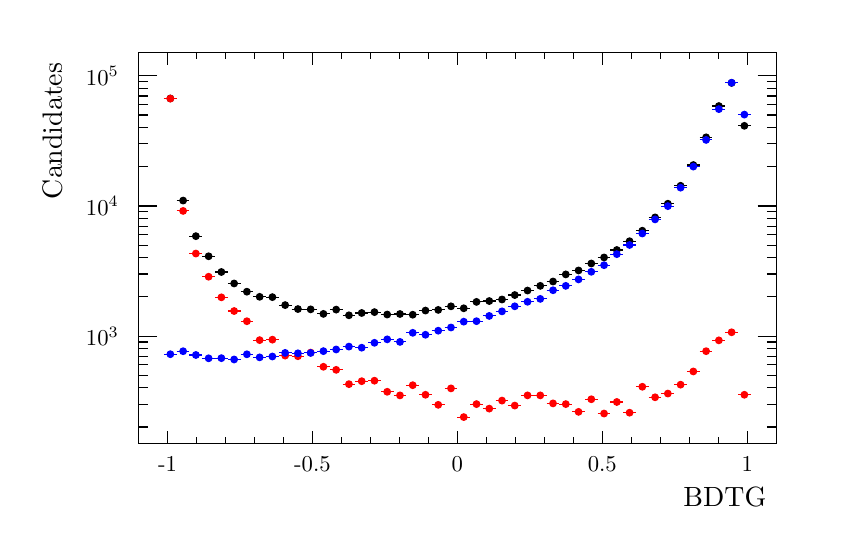
\begin{tikzpicture}
\pgfdeclareplotmark{cross} {
\pgfpathmoveto{\pgfpoint{-0.3\pgfplotmarksize}{\pgfplotmarksize}}
\pgfpathlineto{\pgfpoint{+0.3\pgfplotmarksize}{\pgfplotmarksize}}
\pgfpathlineto{\pgfpoint{+0.3\pgfplotmarksize}{0.3\pgfplotmarksize}}
\pgfpathlineto{\pgfpoint{+1\pgfplotmarksize}{0.3\pgfplotmarksize}}
\pgfpathlineto{\pgfpoint{+1\pgfplotmarksize}{-0.3\pgfplotmarksize}}
\pgfpathlineto{\pgfpoint{+0.3\pgfplotmarksize}{-0.3\pgfplotmarksize}}
\pgfpathlineto{\pgfpoint{+0.3\pgfplotmarksize}{-1.\pgfplotmarksize}}
\pgfpathlineto{\pgfpoint{-0.3\pgfplotmarksize}{-1.\pgfplotmarksize}}
\pgfpathlineto{\pgfpoint{-0.3\pgfplotmarksize}{-0.3\pgfplotmarksize}}
\pgfpathlineto{\pgfpoint{-1.\pgfplotmarksize}{-0.3\pgfplotmarksize}}
\pgfpathlineto{\pgfpoint{-1.\pgfplotmarksize}{0.3\pgfplotmarksize}}
\pgfpathlineto{\pgfpoint{-0.3\pgfplotmarksize}{0.3\pgfplotmarksize}}
\pgfpathclose
\pgfusepathqstroke
}
\pgfdeclareplotmark{cross*} {
\pgfpathmoveto{\pgfpoint{-0.3\pgfplotmarksize}{\pgfplotmarksize}}
\pgfpathlineto{\pgfpoint{+0.3\pgfplotmarksize}{\pgfplotmarksize}}
\pgfpathlineto{\pgfpoint{+0.3\pgfplotmarksize}{0.3\pgfplotmarksize}}
\pgfpathlineto{\pgfpoint{+1\pgfplotmarksize}{0.3\pgfplotmarksize}}
\pgfpathlineto{\pgfpoint{+1\pgfplotmarksize}{-0.3\pgfplotmarksize}}
\pgfpathlineto{\pgfpoint{+0.3\pgfplotmarksize}{-0.3\pgfplotmarksize}}
\pgfpathlineto{\pgfpoint{+0.3\pgfplotmarksize}{-1.\pgfplotmarksize}}
\pgfpathlineto{\pgfpoint{-0.3\pgfplotmarksize}{-1.\pgfplotmarksize}}
\pgfpathlineto{\pgfpoint{-0.3\pgfplotmarksize}{-0.3\pgfplotmarksize}}
\pgfpathlineto{\pgfpoint{-1.\pgfplotmarksize}{-0.3\pgfplotmarksize}}
\pgfpathlineto{\pgfpoint{-1.\pgfplotmarksize}{0.3\pgfplotmarksize}}
\pgfpathlineto{\pgfpoint{-0.3\pgfplotmarksize}{0.3\pgfplotmarksize}}
\pgfpathclose
\pgfusepathqfillstroke
}
\pgfdeclareplotmark{newstar} {
\pgfpathmoveto{\pgfqpoint{0pt}{\pgfplotmarksize}}
\pgfpathlineto{\pgfqpointpolar{44}{0.5\pgfplotmarksize}}
\pgfpathlineto{\pgfqpointpolar{18}{\pgfplotmarksize}}
\pgfpathlineto{\pgfqpointpolar{-20}{0.5\pgfplotmarksize}}
\pgfpathlineto{\pgfqpointpolar{-54}{\pgfplotmarksize}}
\pgfpathlineto{\pgfqpointpolar{-90}{0.5\pgfplotmarksize}}
\pgfpathlineto{\pgfqpointpolar{234}{\pgfplotmarksize}}
\pgfpathlineto{\pgfqpointpolar{198}{0.5\pgfplotmarksize}}
\pgfpathlineto{\pgfqpointpolar{162}{\pgfplotmarksize}}
\pgfpathlineto{\pgfqpointpolar{134}{0.5\pgfplotmarksize}}
\pgfpathclose
\pgfusepathqstroke
}
\pgfdeclareplotmark{newstar*} {
\pgfpathmoveto{\pgfqpoint{0pt}{\pgfplotmarksize}}
\pgfpathlineto{\pgfqpointpolar{44}{0.5\pgfplotmarksize}}
\pgfpathlineto{\pgfqpointpolar{18}{\pgfplotmarksize}}
\pgfpathlineto{\pgfqpointpolar{-20}{0.5\pgfplotmarksize}}
\pgfpathlineto{\pgfqpointpolar{-54}{\pgfplotmarksize}}
\pgfpathlineto{\pgfqpointpolar{-90}{0.5\pgfplotmarksize}}
\pgfpathlineto{\pgfqpointpolar{234}{\pgfplotmarksize}}
\pgfpathlineto{\pgfqpointpolar{198}{0.5\pgfplotmarksize}}
\pgfpathlineto{\pgfqpointpolar{162}{\pgfplotmarksize}}
\pgfpathlineto{\pgfqpointpolar{134}{0.5\pgfplotmarksize}}
\pgfpathclose
\pgfusepathqfillstroke
}
\definecolor{c}{rgb}{1,1,1};
\draw [color=c, fill=c] (0,0) rectangle (10,6.27517);
\draw [color=c, fill=c] (1.4,1.00403) rectangle (9.5,5.96141);
\definecolor{c}{rgb}{0,0,0};
\draw [c] (1.4,1.00403) -- (1.4,5.96141) -- (9.5,5.96141) -- (9.5,1.00403) -- (1.4,1.00403);
\draw [c,line width=0.4] (1.724,5.38328) -- (1.77144,5.38328);
\draw [c,line width=0.4] (1.83856,5.38328) -- (1.886,5.38328);
\foreach \P in {(1.805,5.38328)}{\draw[mark options={color=c,fill=c},mark size=1.201201pt,mark=*] plot coordinates {\P};}
\draw [c,line width=0.4] (1.886,4.08636) -- (1.93344,4.08636);
\draw [c,line width=0.4] (2.00056,4.08636) -- (2.048,4.08636);
\foreach \P in {(1.967,4.08636)}{\draw[mark options={color=c,fill=c},mark size=1.201201pt,mark=*] plot coordinates {\P};}
\draw [c,line width=0.4] (2.048,3.63442) -- (2.09544,3.63442);
\draw [c,line width=0.4] (2.16256,3.63442) -- (2.21,3.63442);
\foreach \P in {(2.129,3.63442)}{\draw[mark options={color=c,fill=c},mark size=1.201201pt,mark=*] plot coordinates {\P};}
\draw [c,line width=0.4] (2.21,3.37898) -- (2.25744,3.37898);
\draw [c,line width=0.4] (2.32456,3.37898) -- (2.372,3.37898);
\foreach \P in {(2.291,3.37898)}{\draw[mark options={color=c,fill=c},mark size=1.201201pt,mark=*] plot coordinates {\P};}
\draw [c,line width=0.4] (2.372,3.17931) -- (2.41944,3.17931);
\draw [c,line width=0.4] (2.48656,3.17931) -- (2.534,3.17931);
\foreach \P in {(2.453,3.17931)}{\draw[mark options={color=c,fill=c},mark size=1.201201pt,mark=*] plot coordinates {\P};}
\draw [c,line width=0.4] (2.534,3.03363) -- (2.58144,3.03363);
\draw [c,line width=0.4] (2.64856,3.03363) -- (2.696,3.03363);
\foreach \P in {(2.615,3.03363)}{\draw[mark options={color=c,fill=c},mark size=1.201201pt,mark=*] plot coordinates {\P};}
\draw [c,line width=0.4] (2.696,2.92906) -- (2.74344,2.92906);
\draw [c,line width=0.4] (2.81056,2.92906) -- (2.858,2.92906);
\foreach \P in {(2.777,2.92906)}{\draw[mark options={color=c,fill=c},mark size=1.201201pt,mark=*] plot coordinates {\P};}
\draw [c,line width=0.4] (2.858,2.86402) -- (2.90544,2.86402);
\draw [c,line width=0.4] (2.97256,2.86402) -- (3.02,2.86402);
\foreach \P in {(2.939,2.86402)}{\draw[mark options={color=c,fill=c},mark size=1.201201pt,mark=*] plot coordinates {\P};}
\draw [c,line width=0.4] (3.02,2.86007) -- (3.06744,2.86007);
\draw [c,line width=0.4] (3.13456,2.86007) -- (3.182,2.86007);
\foreach \P in {(3.101,2.86007)}{\draw[mark options={color=c,fill=c},mark size=1.201201pt,mark=*] plot coordinates {\P};}
\draw [c,line width=0.4] (3.182,2.75887) -- (3.22944,2.75887);
\draw [c,line width=0.4] (3.29656,2.75887) -- (3.344,2.75887);
\foreach \P in {(3.263,2.75887)}{\draw[mark options={color=c,fill=c},mark size=1.201201pt,mark=*] plot coordinates {\P};}
\draw [c,line width=0.4] (3.344,2.70861) -- (3.39144,2.70861);
\draw [c,line width=0.4] (3.45856,2.70861) -- (3.506,2.70861);
\foreach \P in {(3.425,2.70861)}{\draw[mark options={color=c,fill=c},mark size=1.201201pt,mark=*] plot coordinates {\P};}
\draw [c,line width=0.4] (3.506,2.7046) -- (3.55344,2.7046);
\draw [c,line width=0.4] (3.62056,2.7046) -- (3.668,2.7046);
\foreach \P in {(3.587,2.7046)}{\draw[mark options={color=c,fill=c},mark size=1.201201pt,mark=*] plot coordinates {\P};}
\draw [c,line width=0.4] (3.668,2.64734) -- (3.71544,2.64734);
\draw [c,line width=0.4] (3.78256,2.64734) -- (3.83,2.64734);
\foreach \P in {(3.749,2.64734)}{\draw[mark options={color=c,fill=c},mark size=1.201201pt,mark=*] plot coordinates {\P};}
\draw [c,line width=0.4] (3.83,2.70146) -- (3.87744,2.70146);
\draw [c,line width=0.4] (3.94456,2.70146) -- (3.992,2.70146);
\foreach \P in {(3.911,2.70146)}{\draw[mark options={color=c,fill=c},mark size=1.201201pt,mark=*] plot coordinates {\P};}
\draw [c,line width=0.4] (3.992,2.62918) -- (4.03944,2.62918);
\draw [c,line width=0.4] (4.10656,2.62918) -- (4.154,2.62918);
\foreach \P in {(4.073,2.62918)}{\draw[mark options={color=c,fill=c},mark size=1.201201pt,mark=*] plot coordinates {\P};}
\draw [c,line width=0.4] (4.154,2.65888) -- (4.20144,2.65888);
\draw [c,line width=0.4] (4.26856,2.65888) -- (4.316,2.65888);
\foreach \P in {(4.235,2.65888)}{\draw[mark options={color=c,fill=c},mark size=1.201201pt,mark=*] plot coordinates {\P};}
\draw [c,line width=0.4] (4.316,2.66976) -- (4.36344,2.66976);
\draw [c,line width=0.4] (4.43056,2.66976) -- (4.478,2.66976);
\foreach \P in {(4.397,2.66976)}{\draw[mark options={color=c,fill=c},mark size=1.201201pt,mark=*] plot coordinates {\P};}
\draw [c,line width=0.4] (4.478,2.63905) -- (4.52544,2.63905);
\draw [c,line width=0.4] (4.59256,2.63905) -- (4.64,2.63905);
\foreach \P in {(4.559,2.63905)}{\draw[mark options={color=c,fill=c},mark size=1.201201pt,mark=*] plot coordinates {\P};}
\draw [c,line width=0.4] (4.64,2.64588) -- (4.68744,2.64588);
\draw [c,line width=0.4] (4.75456,2.64588) -- (4.802,2.64588);
\foreach \P in {(4.721,2.64588)}{\draw[mark options={color=c,fill=c},mark size=1.201201pt,mark=*] plot coordinates {\P};}
\draw [c,line width=0.4] (4.802,2.6366) -- (4.84944,2.6366);
\draw [c,line width=0.4] (4.91656,2.6366) -- (4.964,2.6366);
\foreach \P in {(4.883,2.6366)}{\draw[mark options={color=c,fill=c},mark size=1.201201pt,mark=*] plot coordinates {\P};}
\draw [c,line width=0.4] (4.964,2.68968) -- (5.01144,2.68968);
\draw [c,line width=0.4] (5.07856,2.68968) -- (5.126,2.68968);
\foreach \P in {(5.045,2.68968)}{\draw[mark options={color=c,fill=c},mark size=1.201201pt,mark=*] plot coordinates {\P};}
\draw [c,line width=0.4] (5.126,2.69785) -- (5.17344,2.69785);
\draw [c,line width=0.4] (5.24056,2.69785) -- (5.288,2.69785);
\foreach \P in {(5.207,2.69785)}{\draw[mark options={color=c,fill=c},mark size=1.201201pt,mark=*] plot coordinates {\P};}
\draw [c,line width=0.4] (5.288,2.74335) -- (5.33544,2.74335);
\draw [c,line width=0.4] (5.40256,2.74335) -- (5.45,2.74335);
\foreach \P in {(5.369,2.74335)}{\draw[mark options={color=c,fill=c},mark size=1.201201pt,mark=*] plot coordinates {\P};}
\draw [c,line width=0.4] (5.45,2.71833) -- (5.49744,2.71833);
\draw [c,line width=0.4] (5.56456,2.71833) -- (5.612,2.71833);
\foreach \P in {(5.531,2.71833)}{\draw[mark options={color=c,fill=c},mark size=1.201201pt,mark=*] plot coordinates {\P};}
\draw [c,line width=0.4] (5.612,2.79959) -- (5.65944,2.79959);
\draw [c,line width=0.4] (5.72656,2.79959) -- (5.774,2.79959);
\foreach \P in {(5.693,2.79959)}{\draw[mark options={color=c,fill=c},mark size=1.201201pt,mark=*] plot coordinates {\P};}
\draw [c,line width=0.4] (5.774,2.81048) -- (5.82144,2.81048);
\draw [c,line width=0.4] (5.88856,2.81048) -- (5.936,2.81048);
\foreach \P in {(5.855,2.81048)}{\draw[mark options={color=c,fill=c},mark size=1.201201pt,mark=*] plot coordinates {\P};}
\draw [c,line width=0.4] (5.936,2.83028) -- (5.98344,2.83028);
\draw [c,line width=0.4] (6.05056,2.83028) -- (6.098,2.83028);
\foreach \P in {(6.017,2.83028)}{\draw[mark options={color=c,fill=c},mark size=1.201201pt,mark=*] plot coordinates {\P};}
\draw [c,line width=0.4] (6.098,2.88659) -- (6.14544,2.88659);
\draw [c,line width=0.4] (6.21256,2.88659) -- (6.26,2.88659);
\foreach \P in {(6.179,2.88659)}{\draw[mark options={color=c,fill=c},mark size=1.201201pt,mark=*] plot coordinates {\P};}
\draw [c,line width=0.4] (6.26,2.94395) -- (6.30744,2.94395);
\draw [c,line width=0.4] (6.37456,2.94395) -- (6.422,2.94395);
\foreach \P in {(6.341,2.94395)}{\draw[mark options={color=c,fill=c},mark size=1.201201pt,mark=*] plot coordinates {\P};}
\draw [c,line width=0.4] (6.422,3.00329) -- (6.46944,3.00329);
\draw [c,line width=0.4] (6.53656,3.00329) -- (6.584,3.00329);
\foreach \P in {(6.503,3.00329)}{\draw[mark options={color=c,fill=c},mark size=1.201201pt,mark=*] plot coordinates {\P};}
\draw [c,line width=0.4] (6.584,3.05837) -- (6.63144,3.05837);
\draw [c,line width=0.4] (6.69856,3.05837) -- (6.746,3.05837);
\foreach \P in {(6.665,3.05837)}{\draw[mark options={color=c,fill=c},mark size=1.201201pt,mark=*] plot coordinates {\P};}
\draw [c,line width=0.4] (6.746,3.14889) -- (6.79344,3.14889);
\draw [c,line width=0.4] (6.86056,3.14889) -- (6.908,3.14889);
\foreach \P in {(6.827,3.14889)}{\draw[mark options={color=c,fill=c},mark size=1.201201pt,mark=*] plot coordinates {\P};}
\draw [c,line width=0.4] (6.908,3.1989) -- (6.95544,3.1989);
\draw [c,line width=0.4] (7.02256,3.1989) -- (7.07,3.1989);
\foreach \P in {(6.989,3.1989)}{\draw[mark options={color=c,fill=c},mark size=1.201201pt,mark=*] plot coordinates {\P};}
\draw [c,line width=0.4] (7.07,3.28736) -- (7.11744,3.28736);
\draw [c,line width=0.4] (7.18456,3.28736) -- (7.232,3.28736);
\foreach \P in {(7.151,3.28736)}{\draw[mark options={color=c,fill=c},mark size=1.201201pt,mark=*] plot coordinates {\P};}
\draw [c,line width=0.4] (7.232,3.36396) -- (7.27944,3.36396);
\draw [c,line width=0.4] (7.34656,3.36396) -- (7.394,3.36396);
\foreach \P in {(7.313,3.36396)}{\draw[mark options={color=c,fill=c},mark size=1.201201pt,mark=*] plot coordinates {\P};}
\draw [c,line width=0.4] (7.394,3.45865) -- (7.44144,3.45865);
\draw [c,line width=0.4] (7.50856,3.45865) -- (7.556,3.45865);
\foreach \P in {(7.475,3.45865)}{\draw[mark options={color=c,fill=c},mark size=1.201201pt,mark=*] plot coordinates {\P};}
\draw [c,line width=0.4] (7.556,3.57029) -- (7.60344,3.57029);
\draw [c,line width=0.4] (7.67056,3.57029) -- (7.718,3.57029);
\foreach \P in {(7.637,3.57029)}{\draw[mark options={color=c,fill=c},mark size=1.201201pt,mark=*] plot coordinates {\P};}
\draw [c,line width=0.4] (7.718,3.70349) -- (7.76544,3.70349);
\draw [c,line width=0.4] (7.83256,3.70349) -- (7.88,3.70349);
\foreach \P in {(7.799,3.70349)}{\draw[mark options={color=c,fill=c},mark size=1.201201pt,mark=*] plot coordinates {\P};}
\draw [c,line width=0.4] (7.88,3.87256) -- (7.92744,3.87256);
\draw [c,line width=0.4] (7.99456,3.87256) -- (8.042,3.87256);
\foreach \P in {(7.961,3.87256)}{\draw[mark options={color=c,fill=c},mark size=1.201201pt,mark=*] plot coordinates {\P};}
\draw [c,line width=0.4] (8.042,4.04625) -- (8.08944,4.04625);
\draw [c,line width=0.4] (8.15656,4.04625) -- (8.204,4.04625);
\foreach \P in {(8.123,4.04625)}{\draw[mark options={color=c,fill=c},mark size=1.201201pt,mark=*] plot coordinates {\P};}
\draw [c,line width=0.4] (8.204,4.27415) -- (8.25144,4.27415);
\draw [c,line width=0.4] (8.31856,4.27415) -- (8.366,4.27415);
\foreach \P in {(8.285,4.27415)}{\draw[mark options={color=c,fill=c},mark size=1.201201pt,mark=*] plot coordinates {\P};}
\draw [c,line width=0.4] (8.366,4.53756) -- (8.41344,4.53756);
\draw [c,line width=0.4] (8.48056,4.53756) -- (8.528,4.53756);
\foreach \P in {(8.447,4.53756)}{\draw[mark options={color=c,fill=c},mark size=1.201201pt,mark=*] plot coordinates {\P};}
\draw [c,line width=0.4] (8.528,4.88958) -- (8.57544,4.88958);
\draw [c,line width=0.4] (8.64256,4.88958) -- (8.69,4.88958);
\foreach \P in {(8.609,4.88958)}{\draw[mark options={color=c,fill=c},mark size=1.201201pt,mark=*] plot coordinates {\P};}
\draw [c,line width=0.4] (8.69,5.28678) -- (8.73744,5.28678);
\draw [c,line width=0.4] (8.80456,5.28678) -- (8.852,5.28678);
\foreach \P in {(8.771,5.28678)}{\draw[mark options={color=c,fill=c},mark size=1.201201pt,mark=*] plot coordinates {\P};}
\draw [c,line width=0.4] (8.852,5.58057) -- (8.89944,5.58057);
\draw [c,line width=0.4] (8.96656,5.58057) -- (9.014,5.58057);
\foreach \P in {(8.933,5.58057)}{\draw[mark options={color=c,fill=c},mark size=1.201201pt,mark=*] plot coordinates {\P};}
\draw [c,line width=0.4] (9.014,5.03564) -- (9.06144,5.03564);
\draw [c,line width=0.4] (9.12856,5.03564) -- (9.176,5.03564);
\foreach \P in {(9.095,5.03564)}{\draw[mark options={color=c,fill=c},mark size=1.201201pt,mark=*] plot coordinates {\P};}
\draw [c,line width=0.4] (1.4,1.00403) -- (9.5,1.00403);
\draw [anchor= east] (9.5,0.317272) node[scale=1.00614, rotate=0]{BDTG};
\draw [c,line width=0.4] (1.76818,1.15651) -- (1.76818,1.00403);
\draw [c,line width=0.4] (2.13636,1.08027) -- (2.13636,1.00403);
\draw [c,line width=0.4] (2.50455,1.08027) -- (2.50455,1.00403);
\draw [c,line width=0.4] (2.87273,1.08027) -- (2.87273,1.00403);
\draw [c,line width=0.4] (3.24091,1.08027) -- (3.24091,1.00403);
\draw [c,line width=0.4] (3.60909,1.15651) -- (3.60909,1.00403);
\draw [c,line width=0.4] (3.97727,1.08027) -- (3.97727,1.00403);
\draw [c,line width=0.4] (4.34545,1.08027) -- (4.34545,1.00403);
\draw [c,line width=0.4] (4.71364,1.08027) -- (4.71364,1.00403);
\draw [c,line width=0.4] (5.08182,1.08027) -- (5.08182,1.00403);
\draw [c,line width=0.4] (5.45,1.15651) -- (5.45,1.00403);
\draw [c,line width=0.4] (5.81818,1.08027) -- (5.81818,1.00403);
\draw [c,line width=0.4] (6.18636,1.08027) -- (6.18636,1.00403);
\draw [c,line width=0.4] (6.55455,1.08027) -- (6.55455,1.00403);
\draw [c,line width=0.4] (6.92273,1.08027) -- (6.92273,1.00403);
\draw [c,line width=0.4] (7.29091,1.15651) -- (7.29091,1.00403);
\draw [c,line width=0.4] (7.65909,1.08027) -- (7.65909,1.00403);
\draw [c,line width=0.4] (8.02727,1.08027) -- (8.02727,1.00403);
\draw [c,line width=0.4] (8.39545,1.08027) -- (8.39545,1.00403);
\draw [c,line width=0.4] (8.76364,1.08027) -- (8.76364,1.00403);
\draw [c,line width=0.4] (9.13182,1.15651) -- (9.13182,1.00403);
\draw [c,line width=0.4] (1.76818,1.15651) -- (1.76818,1.00403);
\draw [c,line width=0.4] (1.4,1.08027) -- (1.4,1.00403);
\draw [c,line width=0.4] (9.13182,1.15651) -- (9.13182,1.00403);
\draw [c,line width=0.4] (9.5,1.08027) -- (9.5,1.00403);
\draw [anchor=base] (1.76818,0.640067) node[scale=0.819821, rotate=0]{-1};
\draw [anchor=base] (3.60909,0.640067) node[scale=0.819821, rotate=0]{-0.5};
\draw [anchor=base] (5.45,0.640067) node[scale=0.819821, rotate=0]{0};
\draw [anchor=base] (7.29091,0.640067) node[scale=0.819821, rotate=0]{0.5};
\draw [anchor=base] (9.13182,0.640067) node[scale=0.819821, rotate=0]{1};
\draw [c,line width=0.4] (1.4,5.96141) -- (9.5,5.96141);
\draw [c,line width=0.4] (1.76818,5.80892) -- (1.76818,5.96141);
\draw [c,line width=0.4] (2.13636,5.88517) -- (2.13636,5.96141);
\draw [c,line width=0.4] (2.50455,5.88517) -- (2.50455,5.96141);
\draw [c,line width=0.4] (2.87273,5.88517) -- (2.87273,5.96141);
\draw [c,line width=0.4] (3.24091,5.88517) -- (3.24091,5.96141);
\draw [c,line width=0.4] (3.60909,5.80892) -- (3.60909,5.96141);
\draw [c,line width=0.4] (3.97727,5.88517) -- (3.97727,5.96141);
\draw [c,line width=0.4] (4.34545,5.88517) -- (4.34545,5.96141);
\draw [c,line width=0.4] (4.71364,5.88517) -- (4.71364,5.96141);
\draw [c,line width=0.4] (5.08182,5.88517) -- (5.08182,5.96141);
\draw [c,line width=0.4] (5.45,5.80892) -- (5.45,5.96141);
\draw [c,line width=0.4] (5.81818,5.88517) -- (5.81818,5.96141);
\draw [c,line width=0.4] (6.18636,5.88517) -- (6.18636,5.96141);
\draw [c,line width=0.4] (6.55455,5.88517) -- (6.55455,5.96141);
\draw [c,line width=0.4] (6.92273,5.88517) -- (6.92273,5.96141);
\draw [c,line width=0.4] (7.29091,5.80892) -- (7.29091,5.96141);
\draw [c,line width=0.4] (7.65909,5.88517) -- (7.65909,5.96141);
\draw [c,line width=0.4] (8.02727,5.88517) -- (8.02727,5.96141);
\draw [c,line width=0.4] (8.39545,5.88517) -- (8.39545,5.96141);
\draw [c,line width=0.4] (8.76364,5.88517) -- (8.76364,5.96141);
\draw [c,line width=0.4] (9.13182,5.80892) -- (9.13182,5.96141);
\draw [c,line width=0.4] (1.76818,5.80892) -- (1.76818,5.96141);
\draw [c,line width=0.4] (1.4,5.88517) -- (1.4,5.96141);
\draw [c,line width=0.4] (9.13182,5.80892) -- (9.13182,5.96141);
\draw [c,line width=0.4] (9.5,5.88517) -- (9.5,5.96141);
\draw [c,line width=0.4] (1.4,1.00403) -- (1.4,5.96141);
\draw [anchor= east] (0.3056,5.96141) node[scale=1.00614, rotate=90]{Candidates};
\draw [c,line width=0.4] (1.5185,1.21048) -- (1.4,1.21048);
\draw [c,line width=0.4] (1.5185,1.50147) -- (1.4,1.50147);
\draw [c,line width=0.4] (1.5185,1.70792) -- (1.4,1.70792);
\draw [c,line width=0.4] (1.5185,1.86806) -- (1.4,1.86806);
\draw [c,line width=0.4] (1.5185,1.99891) -- (1.4,1.99891);
\draw [c,line width=0.4] (1.5185,2.10953) -- (1.4,2.10953);
\draw [c,line width=0.4] (1.5185,2.20536) -- (1.4,2.20536);
\draw [c,line width=0.4] (1.5185,2.28989) -- (1.4,2.28989);
\draw [c,line width=0.4] (1.637,2.3655) -- (1.4,2.3655);
\draw [anchor= east] (1.252,2.3655) node[scale=0.819821, rotate=0]{$10^{3}$};
\draw [c,line width=0.4] (1.5185,2.86294) -- (1.4,2.86294);
\draw [c,line width=0.4] (1.5185,3.15393) -- (1.4,3.15393);
\draw [c,line width=0.4] (1.5185,3.36038) -- (1.4,3.36038);
\draw [c,line width=0.4] (1.5185,3.52052) -- (1.4,3.52052);
\draw [c,line width=0.4] (1.5185,3.65137) -- (1.4,3.65137);
\draw [c,line width=0.4] (1.5185,3.76199) -- (1.4,3.76199);
\draw [c,line width=0.4] (1.5185,3.85782) -- (1.4,3.85782);
\draw [c,line width=0.4] (1.5185,3.94235) -- (1.4,3.94235);
\draw [c,line width=0.4] (1.637,4.01796) -- (1.4,4.01796);
\draw [anchor= east] (1.252,4.01796) node[scale=0.819821, rotate=0]{$10^{4}$};
\draw [c,line width=0.4] (1.5185,4.5154) -- (1.4,4.5154);
\draw [c,line width=0.4] (1.5185,4.80639) -- (1.4,4.80639);
\draw [c,line width=0.4] (1.5185,5.01285) -- (1.4,5.01285);
\draw [c,line width=0.4] (1.5185,5.17299) -- (1.4,5.17299);
\draw [c,line width=0.4] (1.5185,5.30383) -- (1.4,5.30383);
\draw [c,line width=0.4] (1.5185,5.41446) -- (1.4,5.41446);
\draw [c,line width=0.4] (1.5185,5.51029) -- (1.4,5.51029);
\draw [c,line width=0.4] (1.5185,5.59481) -- (1.4,5.59481);
\draw [c,line width=0.4] (1.637,5.67043) -- (1.4,5.67043);
\draw [anchor= east] (1.252,5.67043) node[scale=0.819821, rotate=0]{$10^{5}$};
\draw [c,line width=0.4] (9.5,1.00403) -- (9.5,5.96141);
\draw [c,line width=0.4] (9.3815,1.21048) -- (9.5,1.21048);
\draw [c,line width=0.4] (9.3815,1.50147) -- (9.5,1.50147);
\draw [c,line width=0.4] (9.3815,1.70792) -- (9.5,1.70792);
\draw [c,line width=0.4] (9.3815,1.86806) -- (9.5,1.86806);
\draw [c,line width=0.4] (9.3815,1.99891) -- (9.5,1.99891);
\draw [c,line width=0.4] (9.3815,2.10953) -- (9.5,2.10953);
\draw [c,line width=0.4] (9.3815,2.20536) -- (9.5,2.20536);
\draw [c,line width=0.4] (9.3815,2.28989) -- (9.5,2.28989);
\draw [c,line width=0.4] (9.263,2.3655) -- (9.5,2.3655);
\draw [c,line width=0.4] (9.3815,2.86294) -- (9.5,2.86294);
\draw [c,line width=0.4] (9.3815,3.15393) -- (9.5,3.15393);
\draw [c,line width=0.4] (9.3815,3.36038) -- (9.5,3.36038);
\draw [c,line width=0.4] (9.3815,3.52052) -- (9.5,3.52052);
\draw [c,line width=0.4] (9.3815,3.65137) -- (9.5,3.65137);
\draw [c,line width=0.4] (9.3815,3.76199) -- (9.5,3.76199);
\draw [c,line width=0.4] (9.3815,3.85782) -- (9.5,3.85782);
\draw [c,line width=0.4] (9.3815,3.94235) -- (9.5,3.94235);
\draw [c,line width=0.4] (9.263,4.01796) -- (9.5,4.01796);
\draw [c,line width=0.4] (9.3815,4.5154) -- (9.5,4.5154);
\draw [c,line width=0.4] (9.3815,4.80639) -- (9.5,4.80639);
\draw [c,line width=0.4] (9.3815,5.01285) -- (9.5,5.01285);
\draw [c,line width=0.4] (9.3815,5.17299) -- (9.5,5.17299);
\draw [c,line width=0.4] (9.3815,5.30383) -- (9.5,5.30383);
\draw [c,line width=0.4] (9.3815,5.41446) -- (9.5,5.41446);
\draw [c,line width=0.4] (9.3815,5.51029) -- (9.5,5.51029);
\draw [c,line width=0.4] (9.3815,5.59481) -- (9.5,5.59481);
\draw [c,line width=0.4] (9.263,5.67043) -- (9.5,5.67043);
\definecolor{c}{rgb}{1,0,0};
\draw [c,line width=0.4] (1.724,5.38163) -- (1.77144,5.38163);
\draw [c,line width=0.4] (1.83856,5.38163) -- (1.886,5.38163);
\foreach \P in {(1.805,5.38163)}{\draw[mark options={color=c,fill=c},mark size=1.201201pt,mark=*] plot coordinates {\P};}
\draw [c,line width=0.4] (1.886,3.95491) -- (1.93344,3.95491);
\draw [c,line width=0.4] (2.00056,3.95491) -- (2.048,3.95491);
\foreach \P in {(1.967,3.95491)}{\draw[mark options={color=c,fill=c},mark size=1.201201pt,mark=*] plot coordinates {\P};}
\draw [c,line width=0.4] (2.048,3.41366) -- (2.09544,3.41366);
\draw [c,line width=0.4] (2.16256,3.41366) -- (2.21,3.41366);
\foreach \P in {(2.129,3.41366)}{\draw[mark options={color=c,fill=c},mark size=1.201201pt,mark=*] plot coordinates {\P};}
\draw [c,line width=0.4] (2.21,3.11914) -- (2.25744,3.11914);
\draw [c,line width=0.4] (2.32456,3.11914) -- (2.372,3.11914);
\foreach \P in {(2.291,3.11914)}{\draw[mark options={color=c,fill=c},mark size=1.201201pt,mark=*] plot coordinates {\P};}
\draw [c,line width=0.4] (2.372,2.85749) -- (2.41944,2.85749);
\draw [c,line width=0.4] (2.48656,2.85749) -- (2.534,2.85749);
\foreach \P in {(2.453,2.85749)}{\draw[mark options={color=c,fill=c},mark size=1.201201pt,mark=*] plot coordinates {\P};}
\draw [c,line width=0.4] (2.534,2.68366) -- (2.58144,2.68366);
\draw [c,line width=0.4] (2.64856,2.68366) -- (2.696,2.68366);
\foreach \P in {(2.615,2.68366)}{\draw[mark options={color=c,fill=c},mark size=1.201201pt,mark=*] plot coordinates {\P};}
\draw [c,line width=0.4] (2.696,2.55388) -- (2.74344,2.55388);
\draw [c,line width=0.4] (2.81056,2.55388) -- (2.858,2.55388);
\foreach \P in {(2.777,2.55388)}{\draw[mark options={color=c,fill=c},mark size=1.201201pt,mark=*] plot coordinates {\P};}
\draw [c,line width=0.4] (2.858,2.31411) -- (2.90544,2.31411);
\draw [c,line width=0.4] (2.97256,2.31411) -- (3.02,2.31411);
\foreach \P in {(2.939,2.31411)}{\draw[mark options={color=c,fill=c},mark size=1.201201pt,mark=*] plot coordinates {\P};}
\draw [c,line width=0.4] (3.02,2.32001) -- (3.06744,2.32001);
\draw [c,line width=0.4] (3.13456,2.32001) -- (3.182,2.32001);
\foreach \P in {(3.101,2.32001)}{\draw[mark options={color=c,fill=c},mark size=1.201201pt,mark=*] plot coordinates {\P};}
\draw [c,line width=0.4] (3.182,2.11747) -- (3.22944,2.11747);
\draw [c,line width=0.4] (3.29656,2.11747) -- (3.344,2.11747);
\foreach \P in {(3.263,2.11747)}{\draw[mark options={color=c,fill=c},mark size=1.201201pt,mark=*] plot coordinates {\P};}
\draw [c,line width=0.4] (3.344,2.10962) -- (3.39144,2.10962);
\draw [c,line width=0.4] (3.45856,2.10962) -- (3.506,2.10962);
\foreach \P in {(3.425,2.10962)}{\draw[mark options={color=c,fill=c},mark size=1.201201pt,mark=*] plot coordinates {\P};}
\draw [c,line width=0.4] (3.506,2.15545) -- (3.55344,2.15545);
\draw [c,line width=0.4] (3.62056,2.15545) -- (3.668,2.15545);
\foreach \P in {(3.587,2.15545)}{\draw[mark options={color=c,fill=c},mark size=1.201201pt,mark=*] plot coordinates {\P};}
\draw [c,line width=0.4] (3.668,1.97562) -- (3.71544,1.97562);
\draw [c,line width=0.4] (3.78256,1.97562) -- (3.83,1.97562);
\foreach \P in {(3.749,1.97562)}{\draw[mark options={color=c,fill=c},mark size=1.201201pt,mark=*] plot coordinates {\P};}
\draw [c,line width=0.4] (3.83,1.93655) -- (3.87744,1.93655);
\draw [c,line width=0.4] (3.94456,1.93655) -- (3.992,1.93655);
\foreach \P in {(3.911,1.93655)}{\draw[mark options={color=c,fill=c},mark size=1.201201pt,mark=*] plot coordinates {\P};}
\draw [c,line width=0.4] (4.073,1.71916) -- (4.073,1.7212);
\draw [c,line width=0.4] (4.073,1.78832) -- (4.073,1.78868);
\draw [c,line width=0.4] (3.992,1.75476) -- (4.03944,1.75476);
\draw [c,line width=0.4] (4.10656,1.75476) -- (4.154,1.75476);
\foreach \P in {(4.073,1.75476)}{\draw[mark options={color=c,fill=c},mark size=1.201201pt,mark=*] plot coordinates {\P};}
\draw [c,line width=0.4] (4.235,1.75789) -- (4.235,1.75898);
\draw [c,line width=0.4] (4.154,1.79254) -- (4.20144,1.79254);
\draw [c,line width=0.4] (4.26856,1.79254) -- (4.316,1.79254);
\foreach \P in {(4.235,1.79254)}{\draw[mark options={color=c,fill=c},mark size=1.201201pt,mark=*] plot coordinates {\P};}
\draw [c,line width=0.4] (4.397,1.76415) -- (4.397,1.76509);
\draw [c,line width=0.4] (4.316,1.79865) -- (4.36344,1.79865);
\draw [c,line width=0.4] (4.43056,1.79865) -- (4.478,1.79865);
\foreach \P in {(4.397,1.79865)}{\draw[mark options={color=c,fill=c},mark size=1.201201pt,mark=*] plot coordinates {\P};}
\draw [c,line width=0.4] (4.559,1.61986) -- (4.559,1.62445);
\draw [c,line width=0.4] (4.559,1.69156) -- (4.559,1.69423);
\draw [c,line width=0.4] (4.478,1.65801) -- (4.52544,1.65801);
\draw [c,line width=0.4] (4.59256,1.65801) -- (4.64,1.65801);
\foreach \P in {(4.559,1.65801)}{\draw[mark options={color=c,fill=c},mark size=1.201201pt,mark=*] plot coordinates {\P};}
\draw [c,line width=0.4] (4.721,1.57276) -- (4.721,1.57863);
\draw [c,line width=0.4] (4.721,1.64574) -- (4.721,1.64955);
\draw [c,line width=0.4] (4.64,1.61218) -- (4.68744,1.61218);
\draw [c,line width=0.4] (4.75456,1.61218) -- (4.802,1.61218);
\foreach \P in {(4.721,1.61218)}{\draw[mark options={color=c,fill=c},mark size=1.201201pt,mark=*] plot coordinates {\P};}
\draw [c,line width=0.4] (4.883,1.70578) -- (4.883,1.70816);
\draw [c,line width=0.4] (4.883,1.77527) -- (4.883,1.77593);
\draw [c,line width=0.4] (4.802,1.74171) -- (4.84944,1.74171);
\draw [c,line width=0.4] (4.91656,1.74171) -- (4.964,1.74171);
\foreach \P in {(4.883,1.74171)}{\draw[mark options={color=c,fill=c},mark size=1.201201pt,mark=*] plot coordinates {\P};}
\draw [c,line width=0.4] (5.045,1.58083) -- (5.045,1.58647);
\draw [c,line width=0.4] (5.045,1.65358) -- (5.045,1.6572);
\draw [c,line width=0.4] (4.964,1.62003) -- (5.01144,1.62003);
\draw [c,line width=0.4] (5.07856,1.62003) -- (5.126,1.62003);
\foreach \P in {(5.045,1.62003)}{\draw[mark options={color=c,fill=c},mark size=1.201201pt,mark=*] plot coordinates {\P};}
\draw [c,line width=0.4] (5.207,1.44934) -- (5.207,1.45874);
\draw [c,line width=0.4] (5.207,1.52585) -- (5.207,1.53283);
\draw [c,line width=0.4] (5.126,1.4923) -- (5.17344,1.4923);
\draw [c,line width=0.4] (5.24056,1.4923) -- (5.288,1.4923);
\foreach \P in {(5.207,1.4923)}{\draw[mark options={color=c,fill=c},mark size=1.201201pt,mark=*] plot coordinates {\P};}
\draw [c,line width=0.4] (5.369,1.66409) -- (5.369,1.66752);
\draw [c,line width=0.4] (5.369,1.73464) -- (5.369,1.73626);
\draw [c,line width=0.4] (5.288,1.70108) -- (5.33544,1.70108);
\draw [c,line width=0.4] (5.40256,1.70108) -- (5.45,1.70108);
\foreach \P in {(5.369,1.70108)}{\draw[mark options={color=c,fill=c},mark size=1.201201pt,mark=*] plot coordinates {\P};}
\draw [c,line width=0.4] (5.531,1.28876) -- (5.531,1.30325);
\draw [c,line width=0.4] (5.531,1.37036) -- (5.531,1.38183);
\draw [c,line width=0.4] (5.45,1.3368) -- (5.49744,1.3368);
\draw [c,line width=0.4] (5.56456,1.3368) -- (5.612,1.3368);
\foreach \P in {(5.531,1.3368)}{\draw[mark options={color=c,fill=c},mark size=1.201201pt,mark=*] plot coordinates {\P};}
\draw [c,line width=0.4] (5.693,1.45888) -- (5.693,1.468);
\draw [c,line width=0.4] (5.693,1.53511) -- (5.693,1.54184);
\draw [c,line width=0.4] (5.612,1.50156) -- (5.65944,1.50156);
\draw [c,line width=0.4] (5.72656,1.50156) -- (5.774,1.50156);
\foreach \P in {(5.693,1.50156)}{\draw[mark options={color=c,fill=c},mark size=1.201201pt,mark=*] plot coordinates {\P};}
\draw [c,line width=0.4] (5.855,1.39964) -- (5.855,1.41056);
\draw [c,line width=0.4] (5.855,1.47767) -- (5.855,1.48599);
\draw [c,line width=0.4] (5.774,1.44411) -- (5.82144,1.44411);
\draw [c,line width=0.4] (5.88856,1.44411) -- (5.936,1.44411);
\foreach \P in {(5.855,1.44411)}{\draw[mark options={color=c,fill=c},mark size=1.201201pt,mark=*] plot coordinates {\P};}
\draw [c,line width=0.4] (6.017,1.50481) -- (6.017,1.51259);
\draw [c,line width=0.4] (6.017,1.5797) -- (6.017,1.58523);
\draw [c,line width=0.4] (5.936,1.54615) -- (5.98344,1.54615);
\draw [c,line width=0.4] (6.05056,1.54615) -- (6.098,1.54615);
\foreach \P in {(6.017,1.54615)}{\draw[mark options={color=c,fill=c},mark size=1.201201pt,mark=*] plot coordinates {\P};}
\draw [c,line width=0.4] (6.179,1.43967) -- (6.179,1.44936);
\draw [c,line width=0.4] (6.179,1.51647) -- (6.179,1.52371);
\draw [c,line width=0.4] (6.098,1.48292) -- (6.14544,1.48292);
\draw [c,line width=0.4] (6.21256,1.48292) -- (6.26,1.48292);
\foreach \P in {(6.179,1.48292)}{\draw[mark options={color=c,fill=c},mark size=1.201201pt,mark=*] plot coordinates {\P};}
\draw [c,line width=0.4] (6.341,1.57276) -- (6.341,1.57863);
\draw [c,line width=0.4] (6.341,1.64574) -- (6.341,1.64955);
\draw [c,line width=0.4] (6.26,1.61218) -- (6.30744,1.61218);
\draw [c,line width=0.4] (6.37456,1.61218) -- (6.422,1.61218);
\foreach \P in {(6.341,1.61218)}{\draw[mark options={color=c,fill=c},mark size=1.201201pt,mark=*] plot coordinates {\P};}
\draw [c,line width=0.4] (6.503,1.57276) -- (6.503,1.57863);
\draw [c,line width=0.4] (6.503,1.64574) -- (6.503,1.64955);
\draw [c,line width=0.4] (6.422,1.61218) -- (6.46944,1.61218);
\draw [c,line width=0.4] (6.53656,1.61218) -- (6.584,1.61218);
\foreach \P in {(6.503,1.61218)}{\draw[mark options={color=c,fill=c},mark size=1.201201pt,mark=*] plot coordinates {\P};}
\draw [c,line width=0.4] (6.665,1.4683) -- (6.665,1.47714);
\draw [c,line width=0.4] (6.665,1.54426) -- (6.665,1.55073);
\draw [c,line width=0.4] (6.584,1.5107) -- (6.63144,1.5107);
\draw [c,line width=0.4] (6.69856,1.5107) -- (6.746,1.5107);
\foreach \P in {(6.665,1.5107)}{\draw[mark options={color=c,fill=c},mark size=1.201201pt,mark=*] plot coordinates {\P};}
\draw [c,line width=0.4] (6.827,1.45888) -- (6.827,1.468);
\draw [c,line width=0.4] (6.827,1.53511) -- (6.827,1.54184);
\draw [c,line width=0.4] (6.746,1.50156) -- (6.79344,1.50156);
\draw [c,line width=0.4] (6.86056,1.50156) -- (6.908,1.50156);
\foreach \P in {(6.827,1.50156)}{\draw[mark options={color=c,fill=c},mark size=1.201201pt,mark=*] plot coordinates {\P};}
\draw [c,line width=0.4] (6.989,1.35729) -- (6.989,1.36954);
\draw [c,line width=0.4] (6.989,1.43665) -- (6.989,1.44615);
\draw [c,line width=0.4] (6.908,1.40309) -- (6.95544,1.40309);
\draw [c,line width=0.4] (7.02256,1.40309) -- (7.07,1.40309);
\foreach \P in {(6.989,1.40309)}{\draw[mark options={color=c,fill=c},mark size=1.201201pt,mark=*] plot coordinates {\P};}
\draw [c,line width=0.4] (7.151,1.52241) -- (7.151,1.52968);
\draw [c,line width=0.4] (7.151,1.59679) -- (7.151,1.60186);
\draw [c,line width=0.4] (7.07,1.56323) -- (7.11744,1.56323);
\draw [c,line width=0.4] (7.18456,1.56323) -- (7.232,1.56323);
\foreach \P in {(7.151,1.56323)}{\draw[mark options={color=c,fill=c},mark size=1.201201pt,mark=*] plot coordinates {\P};}
\draw [c,line width=0.4] (7.313,1.33515) -- (7.313,1.34811);
\draw [c,line width=0.4] (7.313,1.41523) -- (7.313,1.42535);
\draw [c,line width=0.4] (7.232,1.38167) -- (7.27944,1.38167);
\draw [c,line width=0.4] (7.34656,1.38167) -- (7.394,1.38167);
\foreach \P in {(7.313,1.38167)}{\draw[mark options={color=c,fill=c},mark size=1.201201pt,mark=*] plot coordinates {\P};}
\draw [c,line width=0.4] (7.475,1.48679) -- (7.475,1.49508);
\draw [c,line width=0.4] (7.475,1.5622) -- (7.475,1.56819);
\draw [c,line width=0.4] (7.394,1.52864) -- (7.44144,1.52864);
\draw [c,line width=0.4] (7.50856,1.52864) -- (7.556,1.52864);
\foreach \P in {(7.475,1.52864)}{\draw[mark options={color=c,fill=c},mark size=1.201201pt,mark=*] plot coordinates {\P};}
\draw [c,line width=0.4] (7.637,1.34631) -- (7.637,1.35891);
\draw [c,line width=0.4] (7.637,1.42602) -- (7.637,1.43583);
\draw [c,line width=0.4] (7.556,1.39246) -- (7.60344,1.39246);
\draw [c,line width=0.4] (7.67056,1.39246) -- (7.718,1.39246);
\foreach \P in {(7.637,1.39246)}{\draw[mark options={color=c,fill=c},mark size=1.201201pt,mark=*] plot coordinates {\P};}
\draw [c,line width=0.4] (7.799,1.68523) -- (7.799,1.68813);
\draw [c,line width=0.4] (7.799,1.75524) -- (7.799,1.75637);
\draw [c,line width=0.4] (7.718,1.72168) -- (7.76544,1.72168);
\draw [c,line width=0.4] (7.83256,1.72168) -- (7.88,1.72168);
\foreach \P in {(7.799,1.72168)}{\draw[mark options={color=c,fill=c},mark size=1.201201pt,mark=*] plot coordinates {\P};}
\draw [c,line width=0.4] (7.961,1.54802) -- (7.961,1.55457);
\draw [c,line width=0.4] (7.961,1.62168) -- (7.961,1.62611);
\draw [c,line width=0.4] (7.88,1.58813) -- (7.92744,1.58813);
\draw [c,line width=0.4] (7.99456,1.58813) -- (8.042,1.58813);
\foreach \P in {(7.961,1.58813)}{\draw[mark options={color=c,fill=c},mark size=1.201201pt,mark=*] plot coordinates {\P};}
\draw [c,line width=0.4] (8.123,1.59669) -- (8.123,1.6019);
\draw [c,line width=0.4] (8.123,1.66902) -- (8.123,1.67224);
\draw [c,line width=0.4] (8.042,1.63546) -- (8.08944,1.63546);
\draw [c,line width=0.4] (8.15656,1.63546) -- (8.204,1.63546);
\foreach \P in {(8.123,1.63546)}{\draw[mark options={color=c,fill=c},mark size=1.201201pt,mark=*] plot coordinates {\P};}
\draw [c,line width=0.4] (8.285,1.7125) -- (8.285,1.71471);
\draw [c,line width=0.4] (8.285,1.78182) -- (8.285,1.78233);
\draw [c,line width=0.4] (8.204,1.74827) -- (8.25144,1.74827);
\draw [c,line width=0.4] (8.31856,1.74827) -- (8.366,1.74827);
\foreach \P in {(8.285,1.74827)}{\draw[mark options={color=c,fill=c},mark size=1.201201pt,mark=*] plot coordinates {\P};}
\draw [c,line width=0.4] (8.366,1.91619) -- (8.41344,1.91619);
\draw [c,line width=0.4] (8.48056,1.91619) -- (8.528,1.91619);
\foreach \P in {(8.447,1.91619)}{\draw[mark options={color=c,fill=c},mark size=1.201201pt,mark=*] plot coordinates {\P};}
\draw [c,line width=0.4] (8.528,2.17371) -- (8.57544,2.17371);
\draw [c,line width=0.4] (8.64256,2.17371) -- (8.69,2.17371);
\foreach \P in {(8.609,2.17371)}{\draw[mark options={color=c,fill=c},mark size=1.201201pt,mark=*] plot coordinates {\P};}
\draw [c,line width=0.4] (8.69,2.31114) -- (8.73744,2.31114);
\draw [c,line width=0.4] (8.80456,2.31114) -- (8.852,2.31114);
\foreach \P in {(8.771,2.31114)}{\draw[mark options={color=c,fill=c},mark size=1.201201pt,mark=*] plot coordinates {\P};}
\draw [c,line width=0.4] (8.852,2.41363) -- (8.89944,2.41363);
\draw [c,line width=0.4] (8.96656,2.41363) -- (9.014,2.41363);
\foreach \P in {(8.933,2.41363)}{\draw[mark options={color=c,fill=c},mark size=1.201201pt,mark=*] plot coordinates {\P};}
\draw [c,line width=0.4] (9.095,1.58083) -- (9.095,1.58647);
\draw [c,line width=0.4] (9.095,1.65358) -- (9.095,1.6572);
\draw [c,line width=0.4] (9.014,1.62003) -- (9.06144,1.62003);
\draw [c,line width=0.4] (9.12856,1.62003) -- (9.176,1.62003);
\foreach \P in {(9.095,1.62003)}{\draw[mark options={color=c,fill=c},mark size=1.201201pt,mark=*] plot coordinates {\P};}
\definecolor{c}{rgb}{0,0,1};
\draw [c,line width=0.4] (1.724,2.13515) -- (1.77144,2.13515);
\draw [c,line width=0.4] (1.83856,2.13515) -- (1.886,2.13515);
\foreach \P in {(1.805,2.13515)}{\draw[mark options={color=c,fill=c},mark size=1.201201pt,mark=*] plot coordinates {\P};}
\draw [c,line width=0.4] (1.886,2.1731) -- (1.93344,2.1731);
\draw [c,line width=0.4] (2.00056,2.1731) -- (2.048,2.1731);
\foreach \P in {(1.967,2.1731)}{\draw[mark options={color=c,fill=c},mark size=1.201201pt,mark=*] plot coordinates {\P};}
\draw [c,line width=0.4] (2.048,2.1252) -- (2.09544,2.1252);
\draw [c,line width=0.4] (2.16256,2.1252) -- (2.21,2.1252);
\foreach \P in {(2.129,2.1252)}{\draw[mark options={color=c,fill=c},mark size=1.201201pt,mark=*] plot coordinates {\P};}
\draw [c,line width=0.4] (2.21,2.08331) -- (2.25744,2.08331);
\draw [c,line width=0.4] (2.32456,2.08331) -- (2.372,2.08331);
\foreach \P in {(2.291,2.08331)}{\draw[mark options={color=c,fill=c},mark size=1.201201pt,mark=*] plot coordinates {\P};}
\draw [c,line width=0.4] (2.372,2.08518) -- (2.41944,2.08518);
\draw [c,line width=0.4] (2.48656,2.08518) -- (2.534,2.08518);
\foreach \P in {(2.453,2.08518)}{\draw[mark options={color=c,fill=c},mark size=1.201201pt,mark=*] plot coordinates {\P};}
\draw [c,line width=0.4] (2.534,2.06815) -- (2.58144,2.06815);
\draw [c,line width=0.4] (2.64856,2.06815) -- (2.696,2.06815);
\foreach \P in {(2.615,2.06815)}{\draw[mark options={color=c,fill=c},mark size=1.201201pt,mark=*] plot coordinates {\P};}
\draw [c,line width=0.4] (2.696,2.13399) -- (2.74344,2.13399);
\draw [c,line width=0.4] (2.81056,2.13399) -- (2.858,2.13399);
\foreach \P in {(2.777,2.13399)}{\draw[mark options={color=c,fill=c},mark size=1.201201pt,mark=*] plot coordinates {\P};}
\draw [c,line width=0.4] (2.858,2.09509) -- (2.90544,2.09509);
\draw [c,line width=0.4] (2.97256,2.09509) -- (3.02,2.09509);
\foreach \P in {(2.939,2.09509)}{\draw[mark options={color=c,fill=c},mark size=1.201201pt,mark=*] plot coordinates {\P};}
\draw [c,line width=0.4] (3.02,2.10608) -- (3.06744,2.10608);
\draw [c,line width=0.4] (3.13456,2.10608) -- (3.182,2.10608);
\foreach \P in {(3.101,2.10608)}{\draw[mark options={color=c,fill=c},mark size=1.201201pt,mark=*] plot coordinates {\P};}
\draw [c,line width=0.4] (3.182,2.15182) -- (3.22944,2.15182);
\draw [c,line width=0.4] (3.29656,2.15182) -- (3.344,2.15182);
\foreach \P in {(3.263,2.15182)}{\draw[mark options={color=c,fill=c},mark size=1.201201pt,mark=*] plot coordinates {\P};}
\draw [c,line width=0.4] (3.344,2.14669) -- (3.39144,2.14669);
\draw [c,line width=0.4] (3.45856,2.14669) -- (3.506,2.14669);
\foreach \P in {(3.425,2.14669)}{\draw[mark options={color=c,fill=c},mark size=1.201201pt,mark=*] plot coordinates {\P};}
\draw [c,line width=0.4] (3.506,2.15126) -- (3.55344,2.15126);
\draw [c,line width=0.4] (3.62056,2.15126) -- (3.668,2.15126);
\foreach \P in {(3.587,2.15126)}{\draw[mark options={color=c,fill=c},mark size=1.201201pt,mark=*] plot coordinates {\P};}
\draw [c,line width=0.4] (3.668,2.1742) -- (3.71544,2.1742);
\draw [c,line width=0.4] (3.78256,2.1742) -- (3.83,2.1742);
\foreach \P in {(3.749,2.1742)}{\draw[mark options={color=c,fill=c},mark size=1.201201pt,mark=*] plot coordinates {\P};}
\draw [c,line width=0.4] (3.83,2.19536) -- (3.87744,2.19536);
\draw [c,line width=0.4] (3.94456,2.19536) -- (3.992,2.19536);
\foreach \P in {(3.911,2.19536)}{\draw[mark options={color=c,fill=c},mark size=1.201201pt,mark=*] plot coordinates {\P};}
\draw [c,line width=0.4] (3.992,2.23185) -- (4.03944,2.23185);
\draw [c,line width=0.4] (4.10656,2.23185) -- (4.154,2.23185);
\foreach \P in {(4.073,2.23185)}{\draw[mark options={color=c,fill=c},mark size=1.201201pt,mark=*] plot coordinates {\P};}
\draw [c,line width=0.4] (4.154,2.218) -- (4.20144,2.218);
\draw [c,line width=0.4] (4.26856,2.218) -- (4.316,2.218);
\foreach \P in {(4.235,2.218)}{\draw[mark options={color=c,fill=c},mark size=1.201201pt,mark=*] plot coordinates {\P};}
\draw [c,line width=0.4] (4.316,2.28001) -- (4.36344,2.28001);
\draw [c,line width=0.4] (4.43056,2.28001) -- (4.478,2.28001);
\foreach \P in {(4.397,2.28001)}{\draw[mark options={color=c,fill=c},mark size=1.201201pt,mark=*] plot coordinates {\P};}
\draw [c,line width=0.4] (4.478,2.3238) -- (4.52544,2.3238);
\draw [c,line width=0.4] (4.59256,2.3238) -- (4.64,2.3238);
\foreach \P in {(4.559,2.3238)}{\draw[mark options={color=c,fill=c},mark size=1.201201pt,mark=*] plot coordinates {\P};}
\draw [c,line width=0.4] (4.64,2.29133) -- (4.68744,2.29133);
\draw [c,line width=0.4] (4.75456,2.29133) -- (4.802,2.29133);
\foreach \P in {(4.721,2.29133)}{\draw[mark options={color=c,fill=c},mark size=1.201201pt,mark=*] plot coordinates {\P};}
\draw [c,line width=0.4] (4.802,2.40688) -- (4.84944,2.40688);
\draw [c,line width=0.4] (4.91656,2.40688) -- (4.964,2.40688);
\foreach \P in {(4.883,2.40688)}{\draw[mark options={color=c,fill=c},mark size=1.201201pt,mark=*] plot coordinates {\P};}
\draw [c,line width=0.4] (4.964,2.38217) -- (5.01144,2.38217);
\draw [c,line width=0.4] (5.07856,2.38217) -- (5.126,2.38217);
\foreach \P in {(5.045,2.38217)}{\draw[mark options={color=c,fill=c},mark size=1.201201pt,mark=*] plot coordinates {\P};}
\draw [c,line width=0.4] (5.126,2.43385) -- (5.17344,2.43385);
\draw [c,line width=0.4] (5.24056,2.43385) -- (5.288,2.43385);
\foreach \P in {(5.207,2.43385)}{\draw[mark options={color=c,fill=c},mark size=1.201201pt,mark=*] plot coordinates {\P};}
\draw [c,line width=0.4] (5.288,2.47449) -- (5.33544,2.47449);
\draw [c,line width=0.4] (5.40256,2.47449) -- (5.45,2.47449);
\foreach \P in {(5.369,2.47449)}{\draw[mark options={color=c,fill=c},mark size=1.201201pt,mark=*] plot coordinates {\P};}
\draw [c,line width=0.4] (5.45,2.54847) -- (5.49744,2.54847);
\draw [c,line width=0.4] (5.56456,2.54847) -- (5.612,2.54847);
\foreach \P in {(5.531,2.54847)}{\draw[mark options={color=c,fill=c},mark size=1.201201pt,mark=*] plot coordinates {\P};}
\draw [c,line width=0.4] (5.612,2.55465) -- (5.65944,2.55465);
\draw [c,line width=0.4] (5.72656,2.55465) -- (5.774,2.55465);
\foreach \P in {(5.693,2.55465)}{\draw[mark options={color=c,fill=c},mark size=1.201201pt,mark=*] plot coordinates {\P};}
\draw [c,line width=0.4] (5.774,2.62116) -- (5.82144,2.62116);
\draw [c,line width=0.4] (5.88856,2.62116) -- (5.936,2.62116);
\foreach \P in {(5.855,2.62116)}{\draw[mark options={color=c,fill=c},mark size=1.201201pt,mark=*] plot coordinates {\P};}
\draw [c,line width=0.4] (5.936,2.67931) -- (5.98344,2.67931);
\draw [c,line width=0.4] (6.05056,2.67931) -- (6.098,2.67931);
\foreach \P in {(6.017,2.67931)}{\draw[mark options={color=c,fill=c},mark size=1.201201pt,mark=*] plot coordinates {\P};}
\draw [c,line width=0.4] (6.098,2.74364) -- (6.14544,2.74364);
\draw [c,line width=0.4] (6.21256,2.74364) -- (6.26,2.74364);
\foreach \P in {(6.179,2.74364)}{\draw[mark options={color=c,fill=c},mark size=1.201201pt,mark=*] plot coordinates {\P};}
\draw [c,line width=0.4] (6.26,2.80106) -- (6.30744,2.80106);
\draw [c,line width=0.4] (6.37456,2.80106) -- (6.422,2.80106);
\foreach \P in {(6.341,2.80106)}{\draw[mark options={color=c,fill=c},mark size=1.201201pt,mark=*] plot coordinates {\P};}
\draw [c,line width=0.4] (6.422,2.83781) -- (6.46944,2.83781);
\draw [c,line width=0.4] (6.53656,2.83781) -- (6.584,2.83781);
\foreach \P in {(6.503,2.83781)}{\draw[mark options={color=c,fill=c},mark size=1.201201pt,mark=*] plot coordinates {\P};}
\draw [c,line width=0.4] (6.584,2.94741) -- (6.63144,2.94741);
\draw [c,line width=0.4] (6.69856,2.94741) -- (6.746,2.94741);
\foreach \P in {(6.665,2.94741)}{\draw[mark options={color=c,fill=c},mark size=1.201201pt,mark=*] plot coordinates {\P};}
\draw [c,line width=0.4] (6.746,3.00313) -- (6.79344,3.00313);
\draw [c,line width=0.4] (6.86056,3.00313) -- (6.908,3.00313);
\foreach \P in {(6.827,3.00313)}{\draw[mark options={color=c,fill=c},mark size=1.201201pt,mark=*] plot coordinates {\P};}
\draw [c,line width=0.4] (6.908,3.08503) -- (6.95544,3.08503);
\draw [c,line width=0.4] (7.02256,3.08503) -- (7.07,3.08503);
\foreach \P in {(6.989,3.08503)}{\draw[mark options={color=c,fill=c},mark size=1.201201pt,mark=*] plot coordinates {\P};}
\draw [c,line width=0.4] (7.07,3.18177) -- (7.11744,3.18177);
\draw [c,line width=0.4] (7.18456,3.18177) -- (7.232,3.18177);
\foreach \P in {(7.151,3.18177)}{\draw[mark options={color=c,fill=c},mark size=1.201201pt,mark=*] plot coordinates {\P};}
\draw [c,line width=0.4] (7.232,3.26556) -- (7.27944,3.26556);
\draw [c,line width=0.4] (7.34656,3.26556) -- (7.394,3.26556);
\foreach \P in {(7.313,3.26556)}{\draw[mark options={color=c,fill=c},mark size=1.201201pt,mark=*] plot coordinates {\P};}
\draw [c,line width=0.4] (7.394,3.40603) -- (7.44144,3.40603);
\draw [c,line width=0.4] (7.50856,3.40603) -- (7.556,3.40603);
\foreach \P in {(7.475,3.40603)}{\draw[mark options={color=c,fill=c},mark size=1.201201pt,mark=*] plot coordinates {\P};}
\draw [c,line width=0.4] (7.556,3.52228) -- (7.60344,3.52228);
\draw [c,line width=0.4] (7.67056,3.52228) -- (7.718,3.52228);
\foreach \P in {(7.637,3.52228)}{\draw[mark options={color=c,fill=c},mark size=1.201201pt,mark=*] plot coordinates {\P};}
\draw [c,line width=0.4] (7.718,3.66824) -- (7.76544,3.66824);
\draw [c,line width=0.4] (7.83256,3.66824) -- (7.88,3.66824);
\foreach \P in {(7.799,3.66824)}{\draw[mark options={color=c,fill=c},mark size=1.201201pt,mark=*] plot coordinates {\P};}
\draw [c,line width=0.4] (7.88,3.8474) -- (7.92744,3.8474);
\draw [c,line width=0.4] (7.99456,3.8474) -- (8.042,3.8474);
\foreach \P in {(7.961,3.8474)}{\draw[mark options={color=c,fill=c},mark size=1.201201pt,mark=*] plot coordinates {\P};}
\draw [c,line width=0.4] (8.042,4.01588) -- (8.08944,4.01588);
\draw [c,line width=0.4] (8.15656,4.01588) -- (8.204,4.01588);
\foreach \P in {(8.123,4.01588)}{\draw[mark options={color=c,fill=c},mark size=1.201201pt,mark=*] plot coordinates {\P};}
\draw [c,line width=0.4] (8.204,4.2502) -- (8.25144,4.2502);
\draw [c,line width=0.4] (8.31856,4.2502) -- (8.366,4.2502);
\foreach \P in {(8.285,4.2502)}{\draw[mark options={color=c,fill=c},mark size=1.201201pt,mark=*] plot coordinates {\P};}
\draw [c,line width=0.4] (8.366,4.518) -- (8.41344,4.518);
\draw [c,line width=0.4] (8.48056,4.518) -- (8.528,4.518);
\foreach \P in {(8.447,4.518)}{\draw[mark options={color=c,fill=c},mark size=1.201201pt,mark=*] plot coordinates {\P};}
\draw [c,line width=0.4] (8.528,4.85675) -- (8.57544,4.85675);
\draw [c,line width=0.4] (8.64256,4.85675) -- (8.69,4.85675);
\foreach \P in {(8.609,4.85675)}{\draw[mark options={color=c,fill=c},mark size=1.201201pt,mark=*] plot coordinates {\P};}
\draw [c,line width=0.4] (8.69,5.24779) -- (8.73744,5.24779);
\draw [c,line width=0.4] (8.80456,5.24779) -- (8.852,5.24779);
\foreach \P in {(8.771,5.24779)}{\draw[mark options={color=c,fill=c},mark size=1.201201pt,mark=*] plot coordinates {\P};}
\draw [c,line width=0.4] (8.852,5.58307) -- (8.89944,5.58307);
\draw [c,line width=0.4] (8.96656,5.58307) -- (9.014,5.58307);
\foreach \P in {(8.933,5.58307)}{\draw[mark options={color=c,fill=c},mark size=1.201201pt,mark=*] plot coordinates {\P};}
\draw [c,line width=0.4] (9.014,5.17823) -- (9.06144,5.17823);
\draw [c,line width=0.4] (9.12856,5.17823) -- (9.176,5.17823);
\foreach \P in {(9.095,5.17823)}{\draw[mark options={color=c,fill=c},mark size=1.201201pt,mark=*] plot coordinates {\P};}
\end{tikzpicture}
